\documentclass[a0paper,portrait]{baposter}



\usepackage{wrapfig}
\usepackage{lmodern}
\usepackage{biblatex}
\usepackage[utf8]{inputenc} %unicode support
\usepackage[T1]{fontenc}
\usepackage{tikzsymbols}
\usepackage[all]{xy}
\usepackage{amsmath}

\usepackage{etoolbox}
\patchcmd{\thebibliography}{\section*{\refname}}{}{}{}


\selectcolormodel{cmyk}

\graphicspath{{figures/}} % Directory in which figures are stored


\newcommand{\compresslist}{%
\setlength{\itemsep}{0pt}%
\setlength{\parskip}{1pt}%
\setlength{\parsep}{0pt}%
}

\newenvironment{boenumerate}
  {\begin{enumerate}\renewcommand\labelenumi{\textbf\theenumi.}}
  {\end{enumerate}}
\renewcommand{\bibname}{BIBLIOGRAPHY}

\begin{document}


\definecolor{darkgreen}{cmyk}{0.8,0,0.8,0.45}
\definecolor{lightgreen}{cmyk}{0.8,0,0.8,0.25}
\definecolor{darkcyan}{HTML}{00838f}
\definecolor{lightcyan}{HTML}{00acc1}

\begin{poster}
{
grid=false,
columns=5,
headerborder=open, % Adds a border around the header of content boxes
colspacing=1em, % Column spacing
bgColorOne=white, % Background color for the gradient on the left side of the poster
bgColorTwo=white, % Background color for the gradient on the right side of the poster
borderColor=darkcyan, % Border color
headerColorOne=lightcyan, % Background color for the header in the content boxes (left side)
headerColorTwo=lightcyan, % Background color for the header in the content boxes (right side)
headerFontColor=white, % Text color for the header text in the content boxes
boxColorOne=white, % Background color of the content boxes
textborder=rounded, %rectangle, % Format of the border around content boxes, can be: none, bars, coils, triangles, rectangle, rounded, roundedsmall, roundedright or faded
eyecatcher=false, % Set to false for ignoring the left logo in the title and move the title left
headerheight=0.11\textheight, % Height of the header
headershape=rounded, % Specify the rounded corner in the content box headers, can be: rectangle, small-rounded, roundedright, roundedleft or rounded
headershade=plain,
headerfont=\Large\textsf, % Large, bold and sans serif font in the headers of content boxes
%textfont={\setlength{\parindent}{1.5em}}, % Uncomment for paragraph indentation
linewidth=2pt % Width of the border lines around content boxes
}
{}
%
%----------------------------------------------------------------------------------------
%	TITLE AND AUTHOR NAME
%----------------------------------------------------------------------------------------
%
{
\textsf{Detección de lenguaje ofensivo con redes neuronales profundas} %Sans Serif
} % Poster title
% {\vspace{1em} Marta Stepniewska, Pawel Siedlecki\\ % Author names
% {\small \vspace{0.7em} Department of Bioinformatics, Institute of Biochemistry and Biophysics, PAS, Warsaw, Pawinskiego 5a}} % Author email addresses
{
\sf\vspace{0.3em}\\
\textbf{Edson Raul Cepeda Marquez}
\vspace{0.1em}\\
\small{Facultad de Ingeniería Mecánica y Eléctrica
\vspace{0.2em}\\
raulcepedac@hotmail.com}
} 
{
\begin{tabular}{l}
     {
\includegraphics[width=40mm]{fime_logo.png}} % University/lab logo \\
     {
\includegraphics[width=40mm]{uanl_logo.png}} % University/lab logo 
\end{tabular}
}



\headerbox{1. Introducción}{name=introduction,column=0,row=0, span=2}{
Uno de los retos actuales de internet es el de mantener las plataformas digitales libres de 
agresiones, mensajes de odio, discriminacion y promover un ambiente sano para los usuarios. 
Las redes sociales son un punto un punto clave para esto puesto que generan una cantidad inmensa de datos que pueden ser utilizados para el estudio e implementación de inteligencia artificial.
El objetivo de este proyecto es identificar correctamente texto con lenguaje ofensivo utilizando técnicas de procesamiento de lenguaje natural y redes neuronales profundas. El enlace al repositorio que contiene el código del proyecto se encuentra en la sección de referencias.
}

\headerbox{2. Herramientas}{name=herramientas, column=0, span=2, below=introduction}{
Se desarrolla código escrito en Python para la resolución de la problemática y se utiliza el entorno de programación Jupyter Notebook. \\

Para el desarrollo de los algoritmos de aprendizage de maquina se hace uso de las librerías Gensim y Keras. Para el control de version se utilza git y repositorios remotos de github. \\

La visualización de datos se realiza con la ayuda de la librería Matplotlib y para la manipulación de los conjuntos de datos Pandas.

Para la documentación se hace uso del sistema de composición de textos LaTex y el editor Overleaf.
\begin{center}

\includegraphics[width=15mm]{480px-Python-logo-notext.svg.png}
\hspace{2mm}

\includegraphics[width=35mm]{gensim.png}
\hspace{2mm}

\includegraphics[width=35mm]{keras.png}
\hspace{2mm}

\includegraphics[width=15mm]{25231.png}

\includegraphics[width=35mm]{pandas.png}

\includegraphics[width=30mm]{latex.png}
\end{center}
}


\headerbox{3. Metodología}{name=metodologia,column=0,span=3,, below=herramientas}{

Se utiliza el conjunto de datos para la identificación de lenguaje ofensivo OLID. Este conjunto de datos contiene 14,100 tweets en ingles etiquetados para entrenamiento y pruebas. 

\begin{center}
\begin{tabular}{| c | c | c | c | c |}
\hline
 id & tweet & a & b & c \\ \hline
86426 & @USER She should ask a few... & OFF & UNT & NaN \\ 
90194 & @USER @USER Go home you’re... & OFF & TIN & NaN \\
16820 & Amazon is investigating... & NOT & Nan & Nan \\ \hline
\end{tabular} \\ 
\end{center}
\begin{center}
\caption{Tabla 1: Conjunto de datos OLID.}
\end{center}

\textbf{Limpieza de datos}: Se realiza una limpieza al conjunto de datos de manera que no exista información innecesaria para el entrenamiento de un algoritmo de aprendizaje automático. Se remueven las etiquetas de id, subtask\_b y subtask\_c. Del texto se eliminan los signos de puntuación, caracteres innecesarios, emoticones y se convierte en minúscula. \\

\textbf{Análisis Exploratorio:} Con la limpieza hecha, se crea uno de los formatos estándar para el análisis, el corpus de texto. Se realiza un conteo de las palabras más frecuentes y se generan nubes de palabras para corroborar que el conjunto de datos tiene sentido y es factible para ser utilizado en un algoritmo.

\begin{center}
    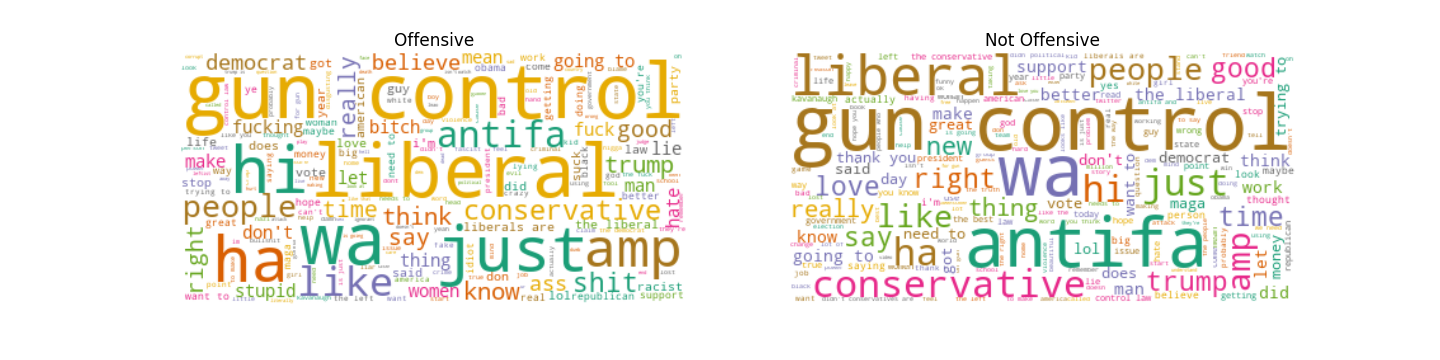
\includegraphics[width=145mm]{word_clouds.png} \\ 
    \caption{Figura 1: Nube de palabras de texto ofensivo y no ofensivo etiquetado en el conjunto de datos.}
\end{center} \\

\textbf{Entrenamiento del algoritmo}: Se entrena un algoritmo de word embeddings para la representación del texto en vectores y se diseña la arquitectura de una red neuronal profunda para la clasificación. 

\begin{center}
\hspace{4cm}
\xymatrix{*+<0.5cm>[F]{Embeddings} \ar[r] & *+<0.5cm>[F]{LSTM} \ar[r] & *+<0.5cm>[F]{Pooling} \ar[r] & *+<0.5cm>[F]{Dropout} \ar[r] & *+<0.5cm>[F]{Densa}} 
\end{center}
\begin{center}
\caption{Figura 2: Arquitectura de la red neuronal.}
\end{center}
} 


\headerbox{4. Resultados}{name=resultados,column=2,span=3}{
Al probar el modelo de word embeddings generado con el corpus de texto es posible buscar similitud de contexto para distintas palabras y realizar operaciones con los vectores de palabras.
\begin{center}
    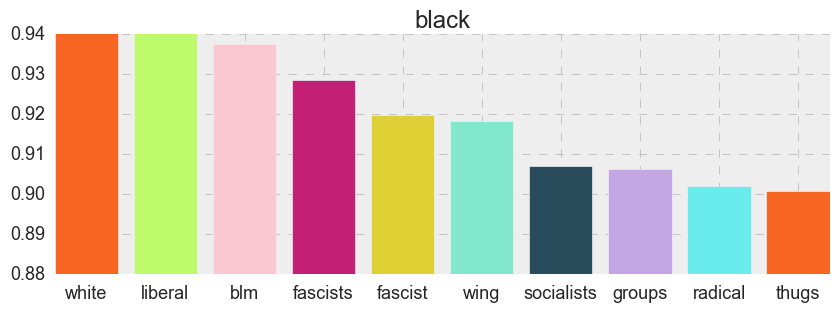
\includegraphics[width=72mm]{barblack.png}
    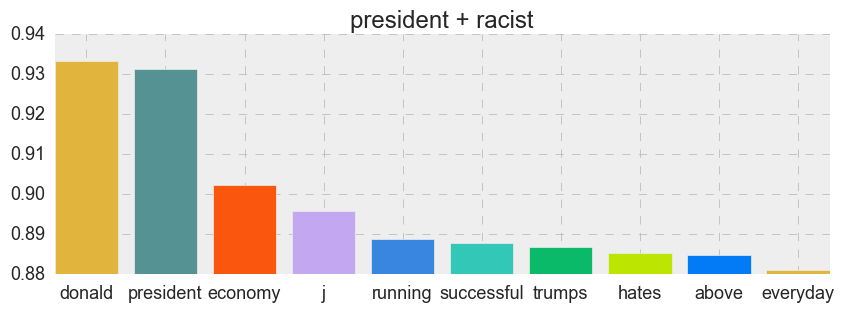
\includegraphics[width=72mm]{barracist.png}
\end{center}
\begin{center}
\caption{Figura 3. Prueba de similaridad en los vectores de palabras.}
\end{center}
Con el word embedding resultante se entrena la red neuronal, se visualiza la variación de la precisión y la perdida y se utiliza la red para realizar predicciones sobre el conjunto de pruebas. Si el valor es mayor a 0.5 se considera ofensivo de otra manera se considera no ofensivo. Parte de las predicciones son las siguientes:
\begin{center}
    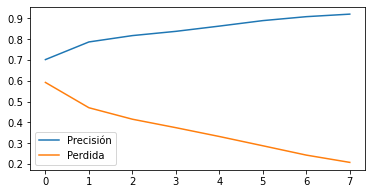
\includegraphics[width=65mm]{precision.png}
\end{center}
\begin{center}
    Figura 4. Variación en la precisión y la perdida de la red neuronal.
\end{center}
\begin{center}
    \begin{tabular}{|c|c|c|}
    \hline
         Texto & Predicción & Esperado \\ \hline
         democrats support antifa muslim brotherhood... ⁦&  [0.996477] & OFF \\
         is revered by conservatives hated by progressives... & [0.029128] & NOT\\
         first it reduces the ca  & [0.082428] & NOT\\
         getting the news that she is still up for parole... &  [0.000400] & NOT\\
         unity demo to oppose the farright in – — enough is enough  &  [0.961980] & OFF\\ \hline
    \end{tabular}
\end{center}
\begin{center}
    \caption{Tabla 2. Predicciones finales de la red.}
\end{center}
}

\headerbox{5. Conclusiones}{name=conclusiones, column=3, span=2, below=resultados}{
Como se puede observar, combinar técnicas de procesamiento de lenguaje natural como word embeddings da un resultado muy positivo combinado con redes neuronales. Especificamente las redes neuronales recurrentes son efectivas para procesar texto puesto que para el análisis contextual es necesario que entradas anteriores afecten a las entradas siguientes, justo lo que sucede en las redes recurrentes LSTM (Long short-term memory). Además los word embeddings no solo sirven para ser la capa de entrada de una red neuronal si no que también permiten crear modelado de temas y modelos de predicciones de palabras.
}

\headerbox{6. Trabajo futuro}{name=tf, column=3, span=2, below=conclusiones}{
Se espera poder trabajar con conjunto de datos más grandes, mejor etiquetados y con una cantidad de características mayor para poder abarcar un mejor vocabulario. Con respecto a los word embeddings se debe utilizar modelos previamente entrenados con conjuntos de datos grandes que dan un mayor rendimiento cuando se usan con redes neuronales. \\\\
Se propone tambíen probar distintas arquitecturas de redes profundas, no solo con redes recurrentes si no también con redes convolucionales.
}
\headerbox{7. Referencias}{name=references,column=3,span=2,below=tf}{


\begin{thebibliography}{9}
    \bibitem{dataset} 
    Zampieri, Marcos and Malmasi, Shervin and Nakov, Preslav and Rosenthal, Sara and Farra, Noura and Kumar, Ritesh.(2019)
    Predicting the Type and Target of Offensive Posts in Social Media.
    Proceedings of NAACL.
    
    \bibitem{kaggle} 
    Bongo. (2020). Do Pretrained Embeddings Give You The Extra Edge? \\
    Recuperado de: \textit{https://www.kaggle.com/sbongo/do-pretrained-embeddings-give-you-the-extra-edge}
    \bibitem{github} 
    Edson Cepeda. (2020). Offensive Language Detection. \\
    \textit{github.com/OrbitalCardinal/OffensiveLanguageDetection}
    
\end{thebibliography}
}

\end{poster}

\end{document}
